\documentclass[12pt]{article}
\usepackage[a4paper, margin=1in]{geometry}

\usepackage{listings}
\usepackage{algorithm}
\usepackage{algpseudocode}

\usepackage{amsmath}
\usepackage{xfrac}
\usepackage{mathtools}
\usepackage{amssymb}
\usepackage{hyperref}
\usepackage{graphicx}
\usepackage{subcaption}

\usepackage{courier}

\lstset{basicstyle=\footnotesize\ttfamily,breaklines=true}

\title{Internship Report}
\date{March 9, 2025}
\author{Aanjishnu Bhattacharyya}

\renewcommand{\thefootnote}{\fnsymbol{footnote}}

\begin{document}

\maketitle
\tableofcontents
\newpage

\section{Introduction}

Numerical Analysis is an very important part of mathematics. It provides us with the tools nessesary to tackle
real-life math problems which are hard to solve analytically. Functions such as the gamma functions and the normal
distribution are extremely difficult to calculate analytically and sometimes impossible. Improper Integrals and
integrals of higher dimentional functions may also be solved in a efficient manner utilizing these methods.

We have tried to build a simple yet powerful software utility which is able to integrate functions with vector valued
inputs and vector valued outputs. It is possible to have multiple nested integrals with varying limits including improper
integrals. Simpsons and Trapezoidal methods are used since they provide a good compromise speed and correctness.
The software utility also provids a rudimentary 3-d visualization framework to plot relevant functions utilizing 3d-acceleration 
hardware present in most modern computers. The software utility also utilizes the feature of runtime link libraries
provided by most modern operating system to provide a seameless user experience.

\section{Learning Phase}

In the learning phase we first develop the mathematical background required for this task.

\subsection{Numerical Method of calculating Integrals}

To compute the integrals of any function, we must first consider the problem of approximating the function.
Approximation in this context reffers to the reconstruction of a function from $n$ sampled points obtained
from the function. This problem becomes much simpler if the sample points are spaced equally apart from eachother.
Fortunately in our particular case we have direct access the the function itself thus it is trivial to obtain such
points. Simpsons method and Trapezoidal method perform the best under these given constraints.
\break
\break

\begin{align*}
	\text{Let, } \quad &f : \mathbb{R} \rightarrow \mathbb{R}\\
			   &f_i = f(x_i) \qquad \forall x_i \in \mathbb{R} \quad \wedge \quad 0 \le i \le n\\\\
	\text{Let, } \quad &L : \mathbb{R} \rightarrow \mathbb{R}\\
		    &L(x) = \sum_{i=0}^n \omega^n_i(x) f_i\\
	&\omega^n_i(x) = \prod \limits_{\substack{j=0 \\ i \not = j}}^n \frac{x - x_j}{x_i - x_j}& \quad i \not = j\\\\
	\text{Now, } \quad &I = \int_{a}^{b} f(x) \mathrm{d}x \qquad \qquad a = \min\{x_i\} \wedge b = \min\{x_i\}\\
				    &= \int_{a}^{b} L(x) \mathrm{d}x\\
				    &= \int_{a}^{b} \sum_{i=0}^n \omega^n_i(x) f_i \mathrm{d}x\\
				    &= \sum_{i=0}^n \int_{a}^{b} \omega^n_i(x) f_i \mathrm{d}x\\
				    &= \sum_{i=0}^n f_i \int_{a}^{b} \prod \limits_{\substack{j=0 \\ i \not = j}}^n \frac{x - x_j}{x_i - x_j} \mathrm{d}x\\\\
	\text{Let, } \quad &h = x_i - x_{i - 1} \qquad \qquad \because x_i\text{ is equispaced}\\
			   &u = \frac{x - x_0}{h}\\
			   &\mathrm{d}u = \frac{1}{h} \mathrm{d}x\\\\
	\text{Substituting }u, \quad &\\
				   &= \sum_{i=0}^n f_i \int_{0}^{n} h \prod \limits_{\substack{j=0 \\ i \not = j}}^n \frac{u - j}{i - j} \mathrm{d}u\\
				   &= \sum_{i=0}^n f_i \frac{h \cdot -1^{n-i}}{i! \cdot (n-i)!} \int_{0}^{n} \prod \limits_{\substack{j=0 \\ i \not = j}}^n {(u - j)} \mathrm{d}u  &\text{\small{(1)}}
\end{align*}

\break
From this general formulae we can derive equations for both Simpsons $(n=2)$ and Trapezoidal $(n=1)$ rules,

\begin{align*}
	\text{From \small{(1)}, } \quad\\
	&I = \sum_{i=0}^n f_i \frac{h \cdot -1^{n-i}}{i! \cdot (n-i)!} \int_{0}^{n} \prod \limits_{\substack{j=0 \\ i \not = j}}^n {(u - j)} \mathrm{d}u\\\\
	\text{For n = 1,}\\
	&= \sum_{i=0}^1 f_i \frac{h \cdot -1^{1-i}}{i! \cdot (1-i)!} \int_{0}^{1} \prod \limits_{\substack{j=0 \\ i \not = j}}^1 {(u - j)} \mathrm{d}u\\\\
	&= -f_0 \cdot h \cdot \int_0^1 (u - 1) \mathrm{d}u + f_1 \cdot h \cdot \int_0^1 u \mathrm{d}u\\
	&= -f_0 \cdot h \cdot \left[ \frac{u^2}{2} - u \right]_0^1 + f_1 \cdot h \cdot \left[\frac{u^2}{2} \right]_0^1\\
	&= (f_0 + f_1) \frac{h}{2}\\\\
	\text{For n = 2,}\\
	&= \sum_{i=0}^2 f_i \frac{h \cdot -1^{2-i}}{i! \cdot (2-i)!} \int_{0}^{2} \prod \limits_{\substack{j=0 \\ i \not = j}}^2 {(u - j)} \mathrm{d}u\\\\
	&= f_0 \cdot h \cdot \int_0^1 (u - 1)(u - 2) \mathrm{d}u - f_1 \cdot h \cdot \int_0^1 u(u - 2) \mathrm{d}u\\
	& \qquad\qquad\qquad\qquad+ f_2 \cdot h \cdot \int_0^1 u(u - 1) \mathrm{d}u\\
	&= (f_0 + 4f_1 + f_2) \frac{h}{3}\\
\end{align*}

\subsection{Integrals with improper limits}

Integrals with improper limits can often be broken down into subpieces which can be computed separately.

e.g,
\begin{equation*}
	\int_{-1}^1 \frac{1}{x} \mathrm{d}x = \lim_{z \rightarrow 0} \left( \int_{-1}^{z} \frac{1}{x} \mathrm{d}x + \int_{z}^{1} \frac{1}{x} \mathrm{d}x \right)
\end{equation*}

We can also have limits which have infinities as their limits, in these cases we can construct a series with
the integrals themselves and try to understand if the series converges. If it does we can also compute for what
values.

e.g,
\begin{equation*}
	\int_{0}^\infty e^{-x^2} \mathrm{d}x\\
\end{equation*}

Let us consider the series,
\begin{equation*}
	S_n = \int_{0}^n e^{-x^2} \mathrm{d}x\\
\end{equation*}

We can say $S_k$ converges if at a large enough value of $k$ equals $S_{k+1}$ given a particular precision.
\begin{equation*}
	S_{n+1} - S_{n} < \vert \epsilon \vert \quad \quad n \ge k \in \mathbb{R}
\end{equation*}

\subsection{Computing Multiple Integrals}

Multiple integrals to compute the volumes and other higher dimentional constructs can be computed through the same methods.
Computing the limits from the outer most integral and then computing limits for these integrals from the inner most integral.
How ever on of the many contrains of this system requires that each limit be defined as a function instead of conditional constraint,
and it may be nesessary to convert conditional constraints into limits

e.g,
\begin{align*}
	&\iint \limits_{x^2 + y^2 \le r^2} f(x, y) \mathrm{d}A\\
	= &\int_{-r}^{r} \left( \int_{-\sqrt{r^2 - y^2}}^{\sqrt{r^2 - y^2}} f(x, y)\mathrm{d}x \right) \mathrm{d}y
\end{align*}

\section{Training}

\subsection{Building an simple prototype of a function integrator and plotter.}

We build a simple prototype\footnote{It is possible to access the prototype from any computer via the internet at: \url{https://nimcompoo-04.github.io/numlysis}}
in javascript to understand how we should aproach building the integrator software\textsuperscript{\ref{fig:prototype1}}.
During this process we avoid using several built in features and external libraries of javascript as to undestand
the internals of such a system and also to keep the program as light weight as possible.

The prototype was capable of integrating any function whose domain was $\mathbb{R}^2$ and range was $\mathbb{R}$.
The interface developed in this prototype resembled that of graphing software desmos. The major things that we learned
from building this prototype were:
\begin{itemize}
	\item The computation time increased rapidly with decrease in the magnitude of $h$ so it was imperative that
		we language which does not have a very high overhead.

	\item We need to separate out the graphing part of the program from the computation part to make it effective and
		fast.

	\item We must allow the user to input data in a known syntax, and allow them to edit the functions at runtime.
\end{itemize}

\begin{figure}
	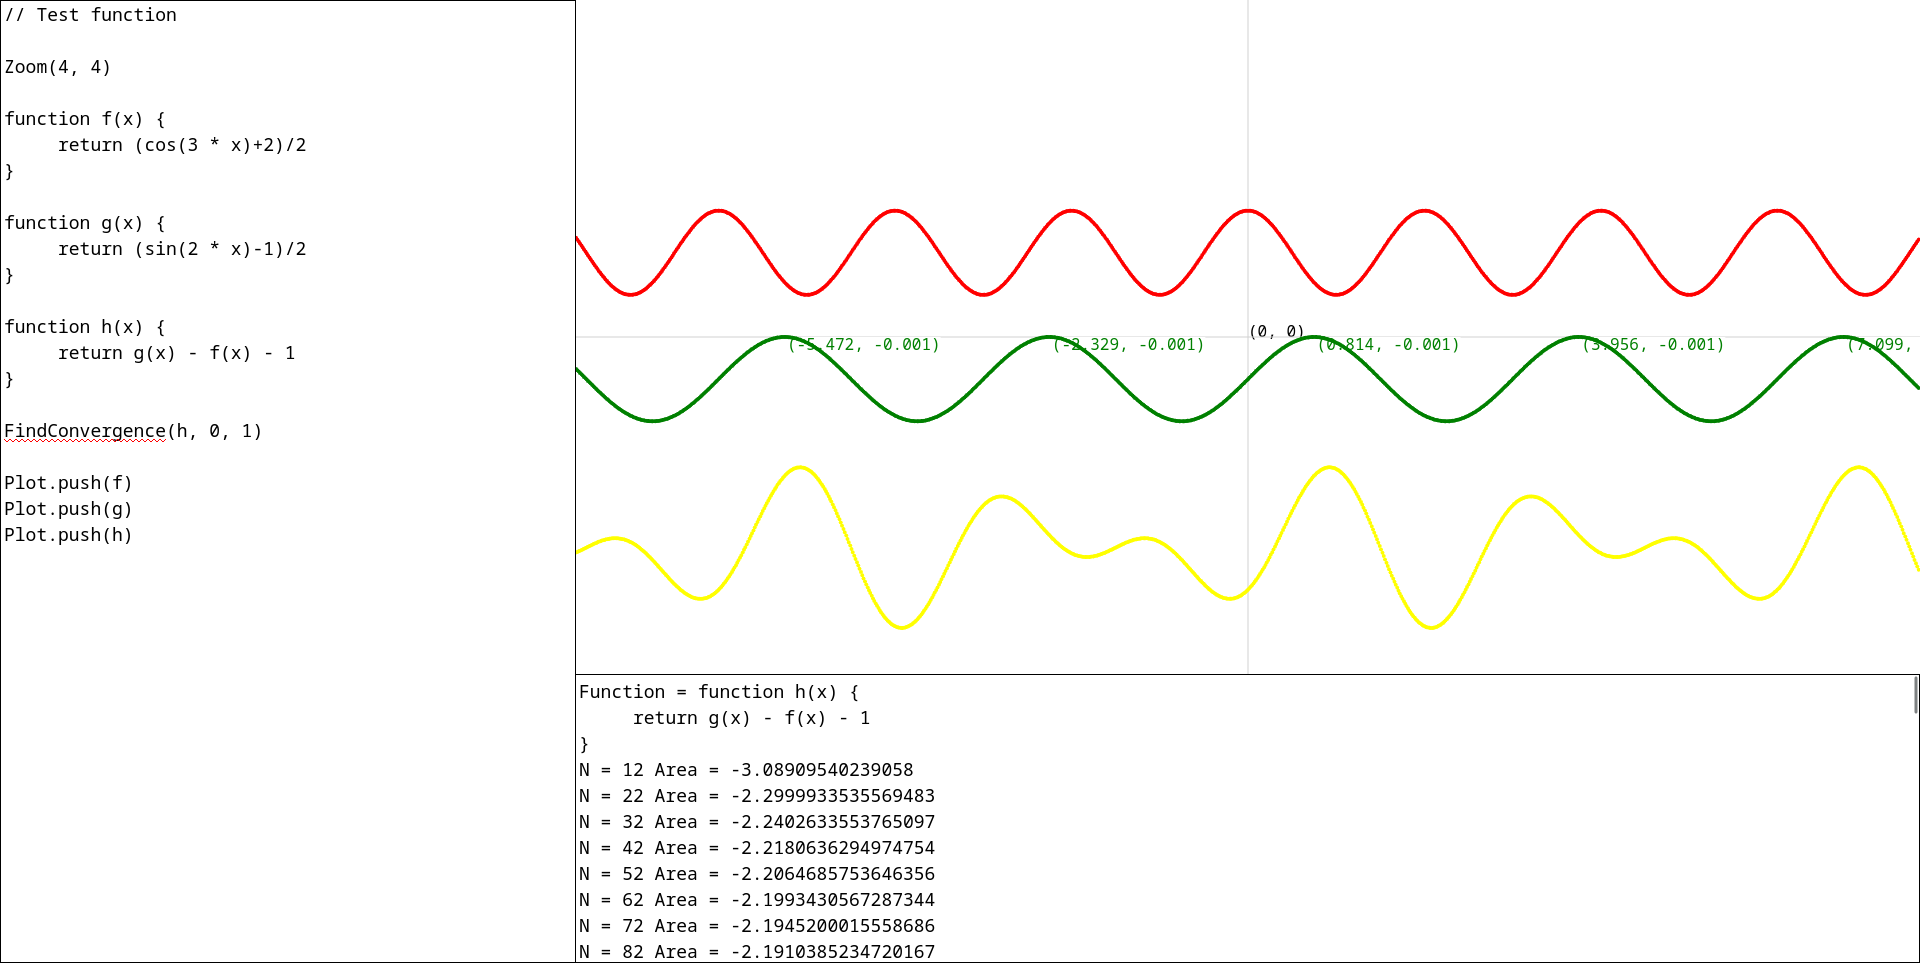
\includegraphics[width=\linewidth]{prototype.png}
	\caption{Integrating and plotting a trigonometric function}
	\label{fig:prototype1}
\end{figure}


\section{Project}

We describe the different parts of the software that we built to implement these numerical methods.

\subsection{Algorithmic approach to numerically solving integrals}

Computing a single integrals is relatively simple. Iteratively we apply trapezoidal or simpson's rule over multiple
samples taken on the function.

\begin{algorithm}
	\caption{Computing an integral of the function $f$.}
	\begin{algorithmic}[1]
		\Procedure{Trapezoidal}{$f_0, f_1$}\Comment{$f_i = f\left(x_i\right)$}
		\State \Return $(f_0 + f_1)/2$
		\EndProcedure
		\Statex
		\Procedure{Integrate}{$s \text{: start}, e \text{: end}, f \text{: function}, n \text{: samples}$}
		\State $h \gets (e - s) / n$
		\State $a \gets 0$\Comment{area under the curve}
		\For{$x \gets s \text{\bf{ to }} e - h \text{\bf{ step }} h$}
		\State $a \gets a + h \cdot Trapezoidal(x, x + h)$
		\EndFor
		\State \Return $a$
		\EndProcedure
	\end{algorithmic}
\end{algorithm}

This is however not very extensible since the function itself is hardcoded to operate on only a single variable. We try
to formulate an extention by which we can reduce the number of inputs the function is operating on.
$$ g(x) = \int_a^b f(x, y) dy $$
We utilize the expression to  extend this algorithm to multiple integrals we devise a simple concept of `context.' `context'
reffers to an associative array which holds the value of all the variables required to compute the function. The sidesteps
the need for positional arguments.

\subsection{Console Interface}

The graphical user interface of the prototype was discarded in favour of a very simple console interface to improve portability of
the software. To provide quality of life features we utilize a console input library Crossline\footnote{Crossline-1.0 Source Code and License: \url{https://github.com/JunchuanWang80/crossline}.}

A part of the user input also involved accepting a C source file which contained all the function expressions. This file is used to allow runtime
expression changing which is further discussed in the later sections.

The users interact with internal integrator using simple commands like `integrate' and `plot'. Commands like `list' and `pointer' were added to 
aid with debugging perposes.

A special set of macros were developed to allow the `list' function to work and to allow a simple way to return vector values.

\subsection{Runtime expression change}

A major problem with our integrator was the slow execution times of a interpreted language. Since each function
had to be executed multiple times the cost of interpreting added up extremely quickly. We noticed this problem in
the prototype, the website would sometimes stop responding due to the high integrator execution times.

To address this problem it was nessesary to compile the expression down to a native binaries which would run orders
of magnitude faster. To achieve this we utilized the very small c99 complient `tiny c compiler'\footnote{Tiny C Compiler Source and License: \url{https://bellard.org/tcc/}}.
We spawned a process with the tcc binaries and compiled the expression C file into a Dynamic link library (or Shared Object).
The generated executable is a Position Independent (reffered to as PIE from here). This allowed use to load this executable at runtime
and execute the native binary version of the expressions. An important factor which allowed this was that all the expressions did not have
any side effects i.e. they did not affect memory of the main process. This meant that we did not have to deal with a situation where the
structure of the code changed but the memory held in the process did not leading to fatal memory corruptions or undefined accesses of memory
locations.

We also considered developing a simple scripting language, but that idea was found to be largly out of the scope of this project.

Some of the hurdles we faced while using the tcc compiler included the lack of support for complex data types which is standard for any c11 compilent
compiler like gcc. We had to implement our own version of complex data type.

\subsection{Multiple Integration}

Functionally Multiple Integrals operate similarly to single integrals as demostrated in previous sections. The way we deal with this in our software is
we have a C structure which represents any given integrals with its limits and the variable it is operating on. We can construct a linked list of such integrals
resolving the limits of each integral from outer outer most to inner most. Then integrating the function from inner to to outer integrals. We also incorportate
a special integral computation module which would allow us to compute integrals of common functions which are known not to behave well under simpsons and 
trapezoidal rule of integration.

\subsection{Plotting of Functions}

Each vector valued function is assumed to be of the form $f:\mathbb{R}^2 \rightarrow \mathbb{R}$ This assumption allows us to plot any given 2d or 1d function.

Values for multiple points are sampled from the function. A group of 3 adjescent points are selected a triangle is formed. In this manner a contiguous mesh of
triangles is generated. each triangle is shaded on the basis of their normal values. The shading gives a sense of depth to the plot. Each point is recomputed each
turn of the plot. To achieve higher resolution plot the number of points sampled is increased.

The triangles are displayed on the screen using the cross platform graphics library Raylib\footnote{Raylib Website: \url{httsp://www.raylib.com}}. Raylib allows a streamlined interfacing with accelerated graphics
hardware using the OpenGL API and a simple way to accept user keyboard input.

\subsection{Special Functions}

Some functions like the gamma function do not behave well with generalized integral computation methods, thus special
methods have been developed to specifically deal with these functions. Currently the only function that has been implemented
under this module is the Gamma function. We utilize the Lanczos Aproximation\cite{aa} for the gamma function to compute their values at 
a resonably high speed and acuracy.

\pagebreak
\subsection{Examples of Function Integration and Plotting}

\subsubsection{Integrating $sin(x)$ function from 0 to $\pi$\textsuperscript{\ref{fig:example1}}}

\begin{flushleft}
Expression C file to integrate sin function from 0 to $\pi$,
\end{flushleft}

\begin{lstlisting}
#include "function.h"

FUNCTION ( X )
vec_t function(vec_t v)
{
	RETURN_VEC ( sin(v.it[0]) );
}

FUNCTION ( )
vec_t limit_start(vec_t v)
{
	RETURN_VEC ( 0 );
}

FUNCTION ( )
vec_t limit_end(vec_t v)
{
	RETURN_VEC( PI );
}
\end{lstlisting}

\begin{flushleft}
Integrating on variable X from 0 to 3.141593.
\end{flushleft}

\begin{center}
	\begin{tabular}{ |c c c c c c| }
		\hline
		\hline
		Step & Variable & $h$ & Start & End & Result \\
		\hline
		\hline
		1 & x & 0.031416 & 0.000000 & 3.141593 & 1.999507 \\
		\hline
		2 & x & 0.030800 & 0.000000 & 3.141593 & 1.999526 \\
		\hline
		3 & x & 0.030208 & 0.000000 & 3.141593 & 1.999544 \\
		\hline
		4 & x & 0.029638 & 0.000000 & 3.141593 & 1.999561 \\
		\hline
		5 & x & 0.029089 & 0.000000 & 3.141593 & 2.000000 \\
		\hline
		6 & x & 0.028560 & 0.000000 & 3.141593 & 2.000000 \\
		\hline
		\hline
	\end{tabular}
\end{center}

\subsubsection{Integrating $sin(x) + sin(y)$ function\textsuperscript{\ref{fig:example2}}}

\begin{flushleft}
Expression C file to integrate $sin(x) + sin(y)$ under the triangle with vertices $(0, 0) (1, 0) (1, 1)$
\end{flushleft}

\begin{lstlisting}
#include "function.h"

FUNCTION  ( X, Y )
vec_t function(vec_t v)
{
	RETURN_VEC ( sin(v.it[0]) + sin(v.it[1]) );
}

FUNCTION ( )
vec_t limit_start_outer (vec_t v)
{
       	RETURN_VEC ( 0 );
}

FUNCTION ( )
vec_t limit_end_outer  (vec_t v)
{
	RETURN_VEC ( 1 );
}

FUNCTION ( )
vec_t limit_start_inner(vec_t v)
{
	RETURN_VEC ( 0 );
}

FUNCTION ( Y )
vec_t limit_end_inner  (vec_t v)
{
	RETURN_VEC ( v.it[0] );
}
\end{lstlisting}

\begin{flushleft}
	Integrating on variable Y then on the inner variable X under the trianglular region with verticles $(0, 0) (1, 0) (1, 1)$
\end{flushleft}

\begin{center}
	\begin{tabular}{ | c c c c c c | }
		\hline
		\hline
		Step & Variable & $h$ & Start & End & Result \\
		\hline
		\hline
		1    & x & 0.000000 & 0.000000 & 0.000167 & 0.000000 \\
		\hline
		2    & x & 0.000000 & 0.000000 & 0.000333 & 0.000000 \\
		\hline
		3    & x & 0.000000 & 0.000000 & 0.000500 & 0.000000 \\
		\hline
		4    & x & 0.000001 & 0.000000 & 0.000667 & 0.000001 \\
		\hline
		5    & x & 0.000001 & 0.000000 & 0.000833 & 0.000001 \\
		\hline
		6    & x & 0.000001 & 0.000000 & 0.001000 & 0.000001 \\
		\hline
		7    & x & 0.000001 & 0.000000 & 0.001000 & 0.000001 \\
		\hline
		8    & x & 0.000001 & 0.000000 & 0.001167 & 0.000002 \\
		\hline
		9    & x & 0.000001 & 0.000000 & 0.001333 & 0.000003 \\
		\hline
		10   & x & 0.000002 & 0.000000 & 0.001500 & 0.000003 \\
		\multicolumn{6}{|c|}{...} \\
		n+1  & x & 0.000999 & 0.000000 & 0.998833 & 1.300255 \\
		\hline
		n+2  & x & 0.000999 & 0.000000 & 0.999000 & 1.300626 \\
		\hline
		n+3  & x & 0.000999 & 0.000000 & 0.999000 & 1.300626 \\
		\hline
		n+4  & x & 0.000999 & 0.000000 & 0.999167 & 1.300997 \\
		\hline
		n+5  & x & 0.000999 & 0.000000 & 0.999333 & 1.299687 \\
		\hline
		n+6  & x & 0.001000 & 0.000000 & 0.999500 & 1.300057 \\
		\hline
		n+7  & x & 0.001000 & 0.000000 & 0.999667 & 1.302110 \\
		\hline
		n+8  & x & 0.001000 & 0.000000 & 0.999833 & 1.302481 \\
		\hline
		n+9  & x & 0.001000 & 0.000000 & 1.000000 & 1.301169 \\
		\hline
		n+10 & y & 0.001000 & 0.000000 & 1.000000 & 0.459997 \\
		\hline
		\hline
	\end{tabular}
\end{center}

\begin{figure}
	\centering
	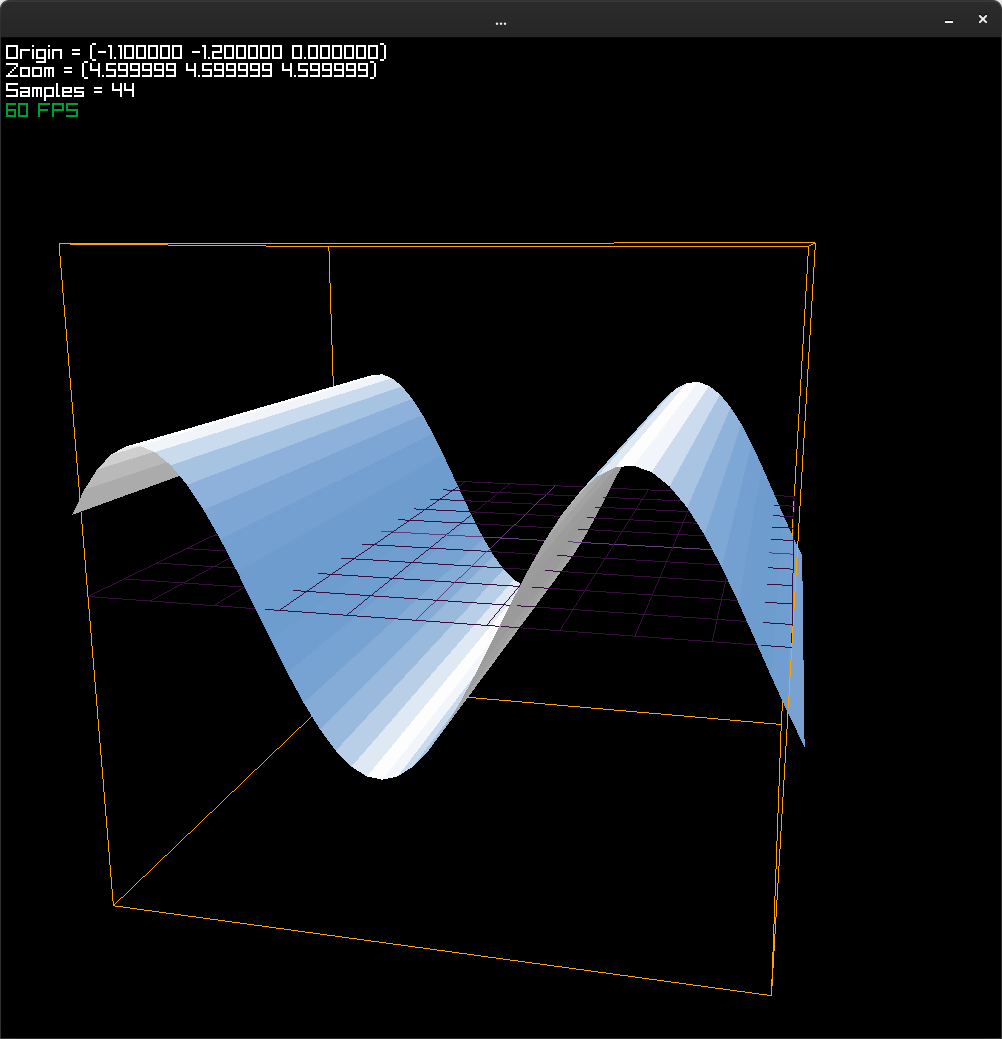
\includegraphics[width=0.65\textwidth]{example1.png}
	\caption{$sin(x)$}
	\label{fig:example1}
\end{figure}

\begin{figure}
	\centering
	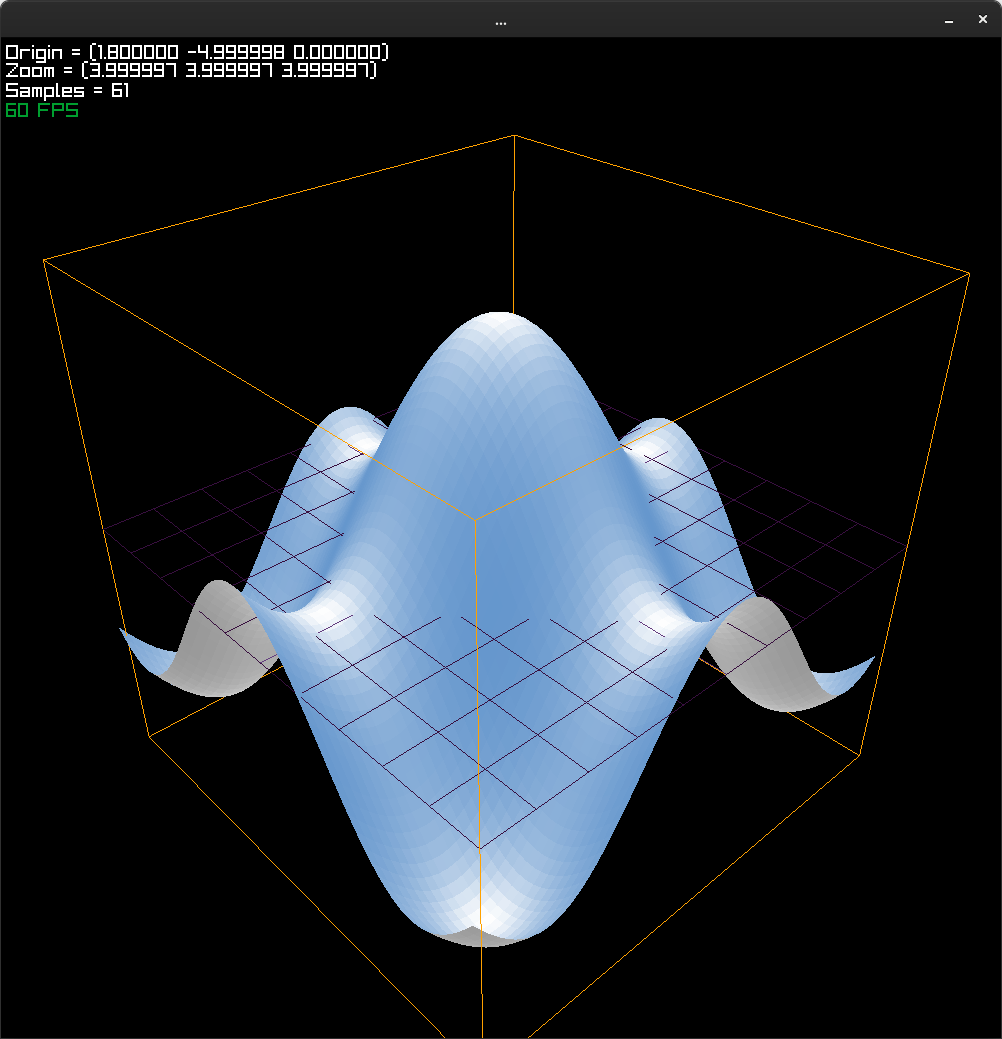
\includegraphics[width=0.65\textwidth]{example2.png}
	\caption{$sin(x) + sin(y)$}
	\label{fig:example2}
\end{figure}

\pagebreak
\section{Results: Computing the value of the Gamma Function numerically}

The gamma function can be defined as,

\begin{align*}
	\Gamma(z) &= \frac{1}{z} \prod_{n = 1}^{\infty} \left[ \frac{1}{1 + \frac{z}{n}} \left(1 + \frac{1}{n} \right)^{z} \right]\\
	\\
	&= \int_0^\infty t^{z-1} e^{-t} dt\\
	\\
	&= z \Gamma(z - 1)
\end{align*}
\\
The gamma function is an relatively difficult function to compute with these simple numerical methods from
a complexity perspective. The major reasons for this being the case are:
\begin{itemize}
	\item The gamma function is computed through an improper integrals.
	\item The function grows at the rate of $O(n!)$ which is very difficult to manage, and precompute.
	\item The function also has discontinuities at the $-ve$ integers
\end{itemize}

To understand the limitations of the program we try to compute and plot the values of the gamma function using
various methods implemented under the plotting and runtime expression compilation tooling we have built.

In the following sections we describe algorithms that have been used to compute the gamma functions. We also
measured the time for computation required to execute these algorithms when implemented under the constraints
of the software we have built. We utilize the implementation of gamma function in pythons math libraries 
to estimate the precision of each method.

\pagebreak
\subsection{Computing values of the Gamma Function using the infinite product definition.}

%\begin{algorithm}
%	\caption{Computing values of the gamma function using Euler infinite product definition}
%	\begin{algorithmic}[1]
%		\Procedure{Gamma}{$z$}\Comment{$z$ is a complex number}
%
%		\State $g \gets 1 / z$
%		\State $n \gets 1$
%
%		\While{$n \le 10^7 $}\Comment{$10^7$ a large number in place of $\infty$}
%
%		\State $a \gets 1 / \left(1 + z / n \right)$
%		\State $b \gets \left(1 + 1 / n \right)^z$
%
%		\State $g \gets g a b$
%		\State $n \gets n + 1$
%
%		\EndWhile
%
%		\State \Return $g$\Comment{result of the gamma function}
%		\EndProcedure
%	\end{algorithmic}
%\end{algorithm}
\begin{center}
	\begin{tabular}{ | c c c c | }
		\hline
		\hline
		Input & Output & Actual & Error\\
		\hline
		\hline
		0.1 & 9.513508 & 9.513507698668732 & 3.0133126749376515e-07\\
		\hline
		0.2 & 4.590844 & 4.5908437119988035 & 2.8800119622474085e-07\\
		\hline
		0.3 & 2.991569 & 2.991568987687591 & 1.2312409314318984e-08\\
		\hline
		0.4 & 2.21816 & 2.2181595437576878 & 4.562423123743997e-07\\
		\hline
		2 & 1.0 & 1.0 & 0.0\\
		\hline
		3 & 1.999999 & 2.0 & -9.999999999177334e-07\\
		\hline
		4 & 5.999996 & 6.0 & -3.9999999996709334e-06\\
		\hline
		5 & 23.999976 & 24.0 & -2.3999999999801958e-05\\
		\hline
		\hline
	\end{tabular}
\end{center}

\subsection{Computing values of the Gamma Function using the Euler integral definition.}

%\begin{algorithm}
%	\caption{Computing values of the gamma function using Euler integral definition}
%	\begin{algorithmic}[1]
%		\Function{F}{$t, z$}\Comment{Function to be integrated}
%		\State $g \gets t^{z - 1}e^{-t}$
%		\State \Return $g$
%		\EndFunction
%\\
%		\Procedure{Gamma}{$z$}\Comment{$z$ is a complex number}
%		\State $I = \int_0^{10^7} F(t, z) dt$\Comment{Integration performed numerically}
%		\State \Return $I$\Comment{$I$ result of integration of $F$}
%		\EndProcedure
%	\end{algorithmic}
%\end{algorithm}
\begin{center}
	\begin{tabular}{ | c c c c | }
		\hline
		\hline
		Input & Output & Actual & Error\\
		\hline
		\hline
		0.1 & 5.625076 & 9.513507698668732 & -3.8884316986687324\\
		\hline
		0.2 & 3.857274 & 4.5908437119988035 & -0.7335697119988036\\
		\hline
		0.3 & 2.811185 & 2.991568987687591 & -0.18038398768759079\\
		\hline
		0.4 & 2.167838 & 2.2181595437576878 & -0.0503215437576876\\
		\hline
		2 & 0.999988 & 1.0 & -1.2000000000012001e-05\\
		\hline
		3 & 2.0 & 2.0 & 0.0\\
		\hline
		4 & 6.0 & 6.0 & 0.0\\
		\hline
		5 & 24.0 & 24.0 & 0.0\\
		\hline
		\hline
	\end{tabular}
\end{center}

\subsection{Computing values of the Gamma Function using the Lanczos approximation.}

\begin{center}
	\begin{tabular}{ | c c c c | }
		\hline
		\hline
		Input & Output & Actual & Error\\
		\hline
		\hline
		0.1 & -9.513508 & 9.513507698668732 & -19.027015698668734\\
		\hline
		0.2 & -4.590844 & 4.5908437119988035 & -9.181687711998803\\
		\hline
		0.3 & -2.991569 & 2.991568987687591 & -5.983137987687591\\
		\hline
		0.4 & -2.21816 & 2.2181595437576878 & -4.436319543757688\\
		\hline
		2 & 1.0 & 1.0 & 0.0\\
		\hline
		3 & 2.0 & 2.0 & 0.0\\
		\hline
		4 & 6.0 & 6.0 & 0.0\\
		\hline
		5 & 24.0 & 24.0 & 0.0\\
		\hline
		\hline
	\end{tabular}
\end{center}

\section{Conclusion}

dfkljdkljadjfaldkjf
adklfjadlfkjlja
aldkjadflj

\section{References}
\begin{thebibliography}{2}
	\bibitem{aa} Godfrey, Paul (2001). "Lanczos Implementation of the Gamma Function" \url{http://www.numericana.com/answer/info/godfrey.htm}
\end{thebibliography}

\end{document}
